\documentclass[11pt,a4paper]{report}

% --- PAQUETES NECESARIOS ---
\usepackage[utf8]{inputenc}
\usepackage[spanish, es-tabla]{babel}
\usepackage[most]{tcolorbox} 
\usepackage{fontawesome5}    
\usepackage{enumitem}       
\usepackage{graphicx}       
\usepackage{geometry}
\usepackage[hidelinks]{hyperref}
\usepackage{caption} % Para manejar mejor los pies de foto
\usepackage{qrcode}  % Opcional, si quieres que LaTeX genere el QR por ti
\usepackage{titlesec}
\geometry{margin=2.5cm}

% Títulos compactos para dejar espacio a la primera receta de cada capítulo.
\titlespacing*{\chapter}{0pt}{-30pt}{14pt}

% --- DEFINICIÓN DEL ESTILO DE LA RECETA CORREGIDO ---
\newtcolorbox{receta}[2]{
    enhanced,
    colback=white,
    colframe=orange!80!black,
    fonttitle=\bfseries\Large,
    title={\faUtensils\ #1 \hfill \faClock\ #2},
    % En lugar de 'no hyperref', usamos esto para evitar el conflicto
    hypertarget={receta#1}, 
    attach boxed title to top center={yshift=-3mm},
    boxed title style={colback=orange!80!black, sharp corners},
    sharp corners,
    drop shadow,
    % Quitamos el 'code' que añade al índice desde aquí 
    before skip=12pt,
    after skip=0pt
}

% --- COMANDO PARA EL ÍNDICE Y REFERENCIAS SIN WARNINGS ---
\newcommand{\nuevaReceta}[3]{% 
    \phantomsection % Crea el ancla para el índice y hyperref
    \addcontentsline{toc}{section}{#1}% Registra en el índice
    \begin{receta}{#1}{#2}% Abre la caja (Título y Tiempo)
    \label{#3}% Establece la etiqueta para usar con \pageref
}

% --- IMÁGENES DE RECETA COMPLETAS ---
% El argumento opcional adapta el ancho al espacio disponible en cada receta.
\newcommand{\imagenReceta}[3][0.64]{%
    \begin{center}
        \includegraphics[width=#1\textwidth]{#2}%
        \\ \vspace{0.3em}
        \small \textit{#3}
    \end{center}
    \vspace{0.2em}%
}

% Cada cuadro comienza donde haya espacio suficiente y termina la página.
\newcommand{\recetaPaginaCompleta}[1]{%
    \input{#1}%
    \clearpage
}

% --- INICIO DEL DOCUMENTO ---
\begin{document}

    \newsavebox{\miqrMexicano}
    \sbox{\miqrMexicano}{\qrcode[height=1.5cm]{https://open.spotify.com/playlist/6XOkYG9TT3Scvs9rsZ0xZF}}

\hypersetup{pageanchor=false}
\begin{titlepage}
    \centering
    \vspace*{1cm}
    {\Huge \textbf{Si esto compila, se come}} \\
    \vspace{0.8cm}
    {\Large \textit{Recetas hechas con amor y \LaTeX\ }}
    
    \vspace{1cm}
    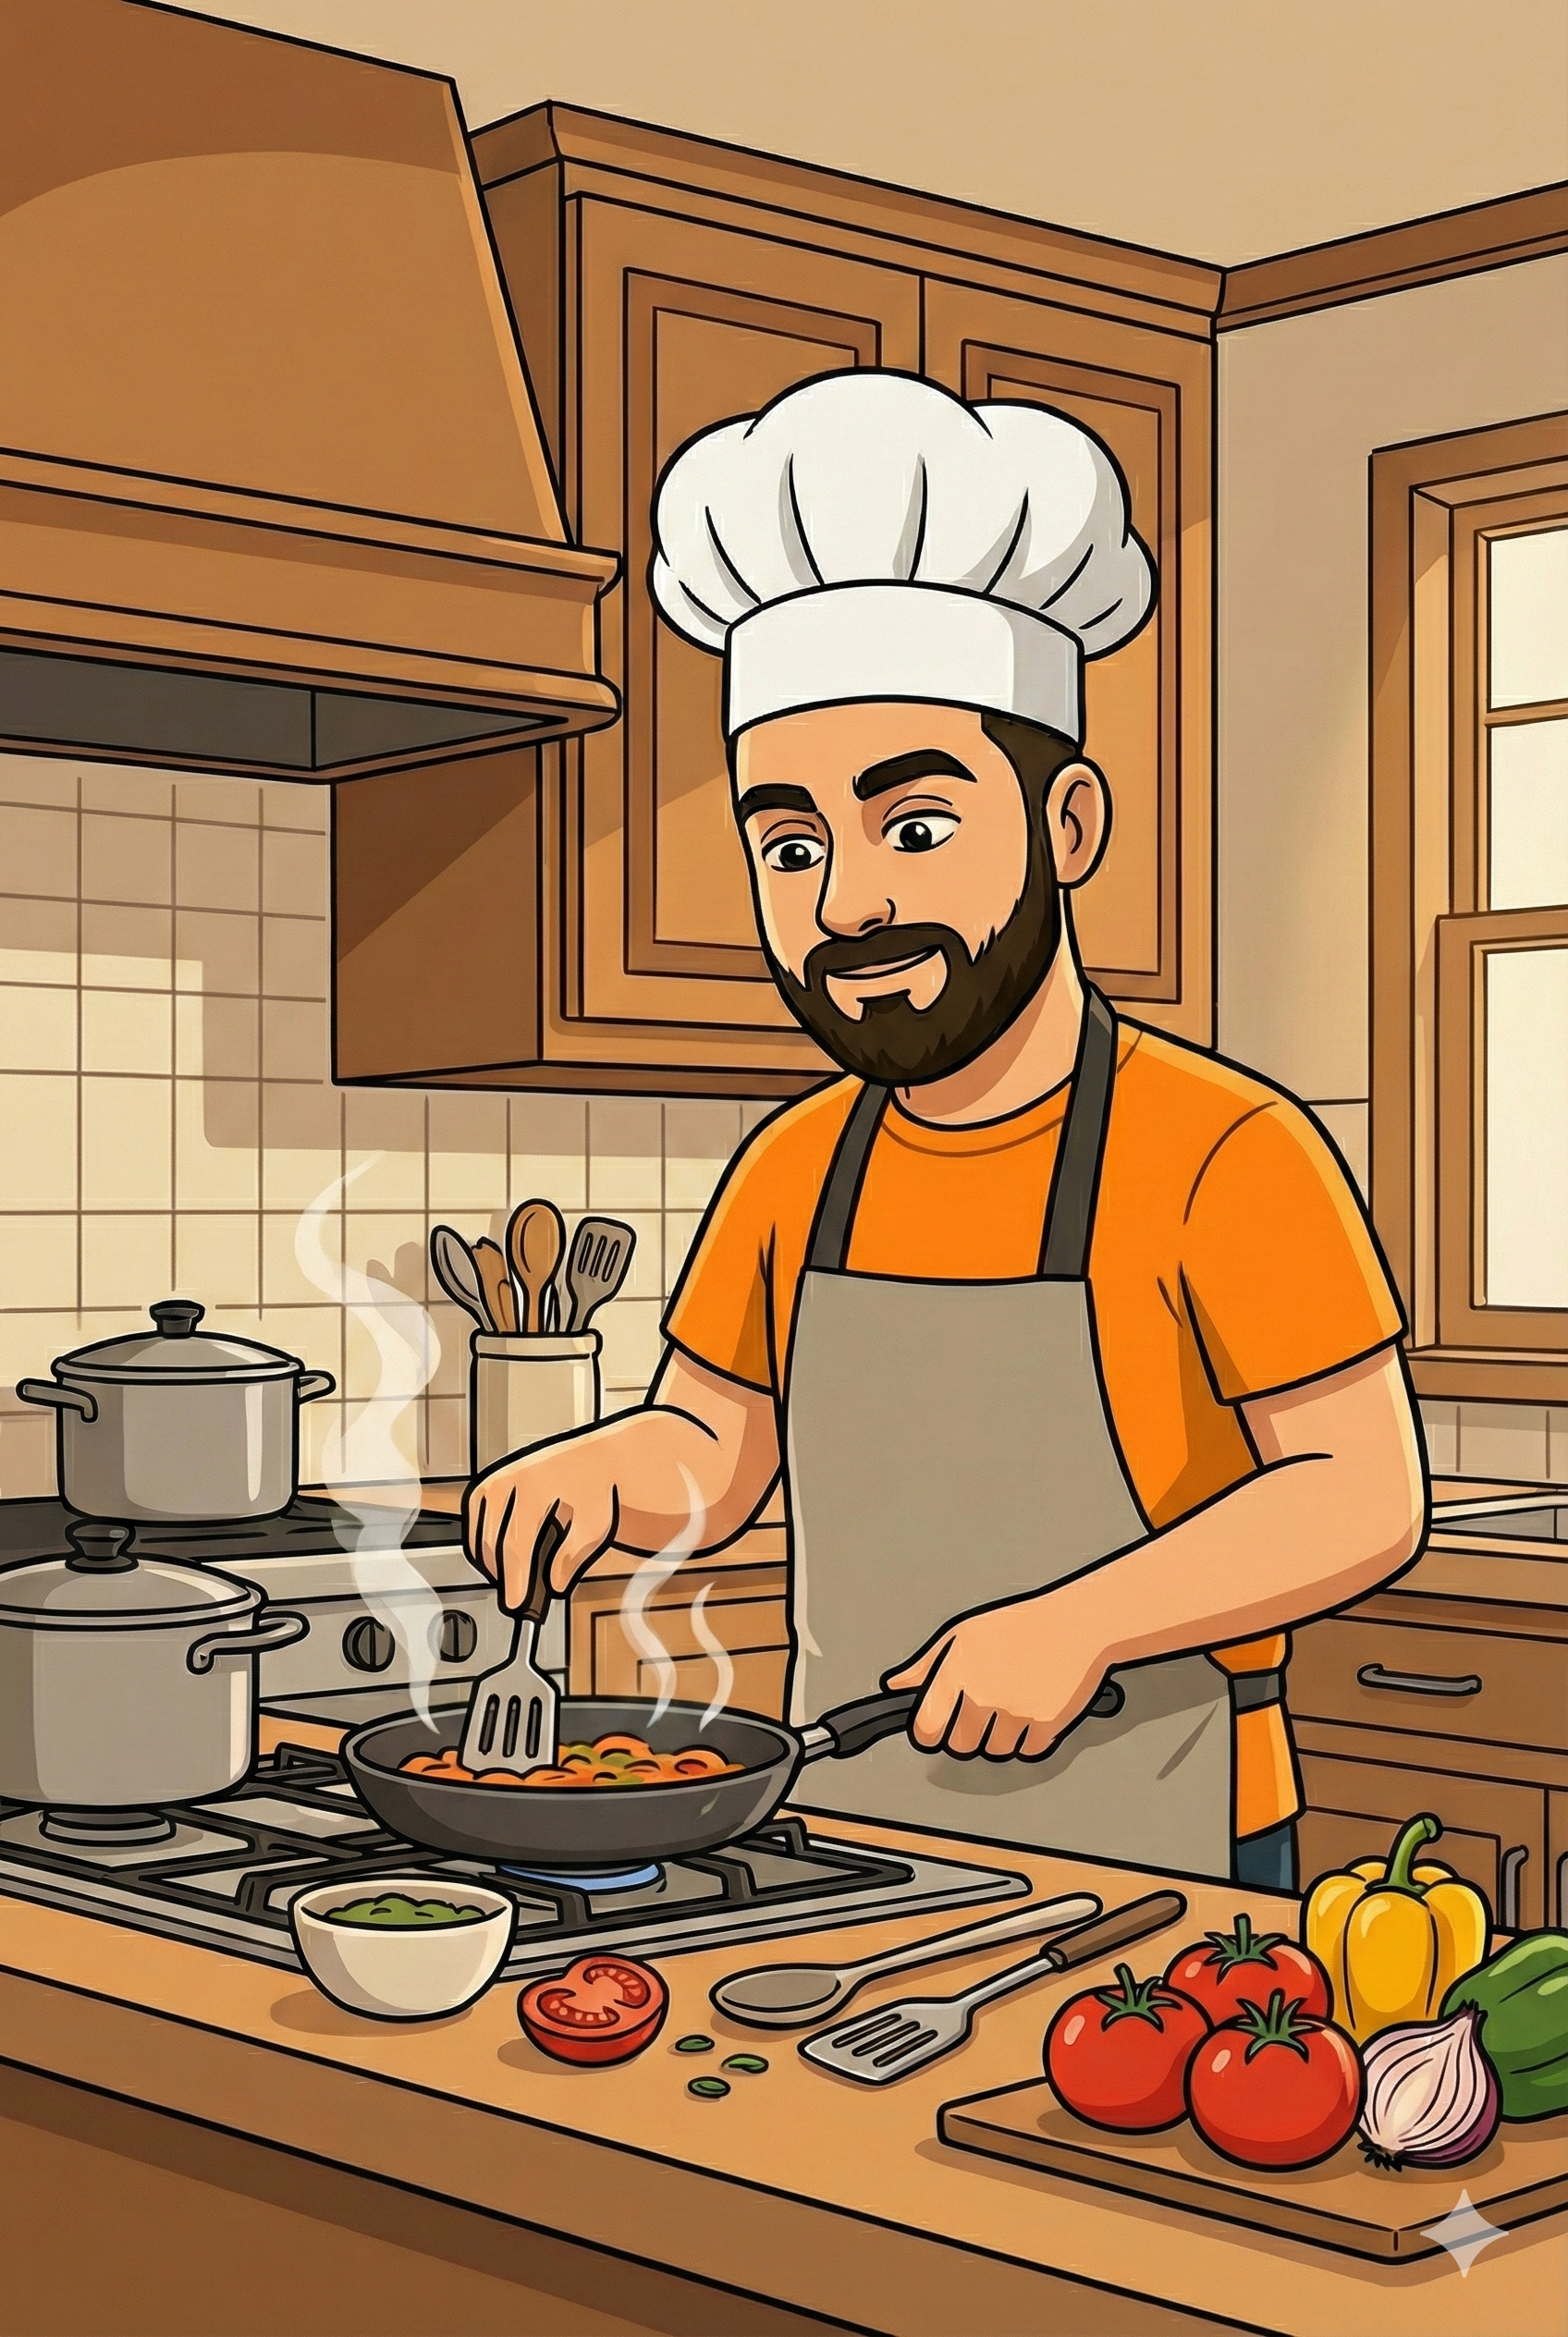
\includegraphics[width=0.55\textwidth]{imagenes/portada.png}
    
    \vfill
    {\Large \faUtensils \ \today} \\ % Aquí hemos borrado el 
    \vspace{0.5cm}
\end{titlepage}
\hypersetup{pageanchor=true}

\tableofcontents 
\newpage

\chapter{Entrantes y Aperitivos}
\recetaPaginaCompleta{secciones/entrantes/guacamole.tex}
\recetaPaginaCompleta{secciones/entrantes/salmorejo.tex}

\chapter{Platos Principales}
\recetaPaginaCompleta{secciones/principales/guisillo.tex}
\recetaPaginaCompleta{secciones/principales/remojon.tex}
\recetaPaginaCompleta{secciones/principales/fideos.tex}
\recetaPaginaCompleta{secciones/principales/arroz_lena.tex}
\recetaPaginaCompleta{secciones/principales/tacos_entrana.tex}
\recetaPaginaCompleta{secciones/principales/sopa_miso.tex}
\recetaPaginaCompleta{secciones/principales/asado_versatil.tex}
\recetaPaginaCompleta{secciones/principales/fajitas.tex}

\chapter{Postres}
\recetaPaginaCompleta{secciones/postres/mousse_limon.tex}

\end{document}
